\subsection{Identifikasi Komponen Fundamental}
	Berdasarkan Bab Analisa, dapat diidentifikasi dan divisualisasikan pada Gambar \ref{fundamental-component} yaitu komponen-komponen penting dalam pembuatan aplikasi sebagai berikut:
	\begin{enumerate}
		\item Web Server 
		\item Mekanisme penyimpanan data (\textit{database} dan \textit{data storage})
		\item \textit{User Interface} sebagai media terhadap \textit{end-user}
		\item Mekanisme Asinkronus untuk mengakomodasi fitur \textit{realtime}
	\end{enumerate}
	
	\begin{figure}[H]
		\centering
		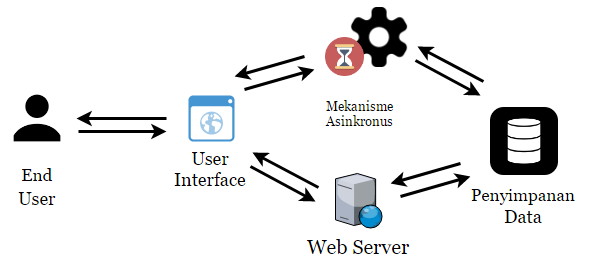
\includegraphics
		[width=\textwidth]
		{images/bab3/buku/basic_architecture.png}
		\caption{Arsitektur dasar yang dibutuhkan untuk membangun aplikasi}
		\label{fundamental-component}
	\end{figure}
	
	
